\documentclass{article}

\usepackage[T1]{fontenc}
\usepackage{mathptmx}
\usepackage{setspace}
\usepackage[top=1in,bottom=1in,left=3cm,right=2.4cm]{geometry}
\usepackage{listings}
\usepackage{graphicx}
\usepackage{subcaption}
\usepackage[sort&compress]{natbib}
\usepackage{hyperref}
\hypersetup{
	colorlinks,
	linkcolor=red,
	urlcolor=blue
}
\urlstyle{same}


\begin{document}
	\title{Intermediate report with \LaTeX} 
	\author{Bey Nesrine, Gresh Clément}
	
	\date{Université de Paris \\[5mm]February 16, 2022 }
	
	\maketitle
	
	\tableofcontents\hrule
	
	\section{ General Presentation }\label{sec:first}
	this project is about identifying Sign Language Movements made in front of a camera and translating them into a readable or hearable wording.
	
	
	Thanks to \textbf{Opencv} and \textbf{MediaPipe} it was simple to identify the landmarks on the hands and to aknowledge the data and process it in order to store the positioning of each landmark with its exact coordinates.
	
	As shown in Figure 1, the figertips are easily recognized and their positioning can be determined depending on other marks on the same finger, in order to know whether the finger is closed or not, whether it is on left side or the right one (concerns the opening and closing of thumbs only).
	
	if you would like to know more about MediaPipe click \href{https://mediapipe.dev/}{here}.
	
	\hrule
	\begin{figure}[h!]
		\center
		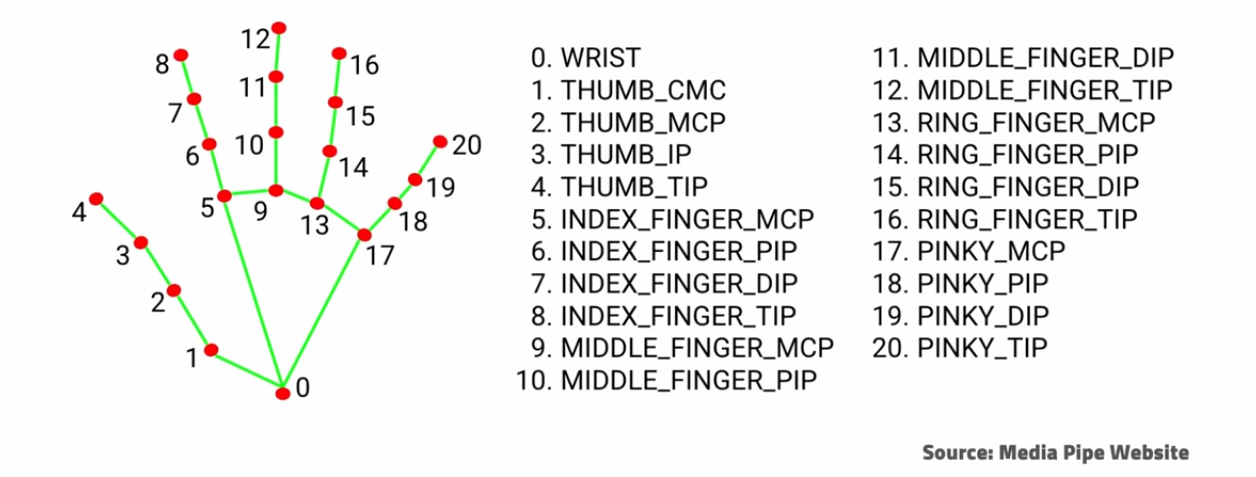
\includegraphics[width=\linewidth]{landmarks.png}
		\caption{ hand landmarks}
	\end{figure}
\hrule
	\section{Advancement Description}\label{sec:second}
	Currently our code can determine the hand positioning as well as a specific fingertip's coordinates, it then can tell which letter of the \textbf{Sign Language Alphabet} it is,we have decided to work on different branches where one consits of using predefined methods and classes and the other aims to write the methods that can do the equivelent tasks.
	
	We will incorporate some code samples and images of how it can recognize, we still haven't developed an efficient Artificial Intelligence but we'll enlighten you about it in the next content.
	The following portion of the code shows a sample of the module that identifies letters efficiently.
	\renewcommand\lstlistingname{Source code}
\renewcommand\lstlistlistingname{Source code}
\begin{lstlisting}[language=python,caption={Naive Hand Recognition},breaklines=true]
		while True:
	success, img = cap.read()
	img = detector.hand_detection(img)
	lmList = detector.find_position(img, draw=False)
	# print(lmList)
	if len(lmList) != 0:
	fingerPos = []
	# thumb
	if lmList[fingerTips[0]][1] > lmList[fingerTips[0] - 1][1]:  # 1 refers t x
	fingerPos.append(1)
	else:
	fingerPos.append(0)
	
	# 4 finger
	for i in range(1, 5):
	if lmList[fingerTips[i]][2] < lmList[fingerTips[i]-2][2]:  # 2 refers t y
	fingerPos.append(1)
	else:
	fingerPos.append(0)
	for i in range(0, 5):
	if fingerPos[0] == 0 and fingerPos[1] == 1 and fingerPos[2] == 1 and fingerPos[3] == 1 \
	and fingerPos[4] == 1:
	print("C'est la lettre B de l'alphabet!")
	elif fingerPos[0] == 1 and fingerPos[1] == 0 and fingerPos[2] == 0 and fingerPos[3] == 0 \
	and fingerPos[4] == 0:
	print("C'est la lettre A de l'alphabet!")
	elif fingerPos[0] == 0 and fingerPos[1] == 0 and fingerPos[2] == 0 and fingerPos[3] == 0 \
	and fingerPos[4] == 0:
	print("C'est la lettre E de l'alphabet! ")
	elif fingerPos[0] == 0 and fingerPos[1] == 0 and fingerPos[2] == 1 and fingerPos[3] == 1 \
	and fingerPos[4] == 1:
	print("C'est la lettre F de l'alphabet! ")
	elif fingerPos[0] == 0 and fingerPos[1] == 1 and fingerPos[2] == 1 and fingerPos[3] == 0 \
	and fingerPos[4] == 0:
	print("C'est la lettre U de l'alphabet!")
\end{lstlisting}	
	
	\section{Developement And Difficulties}\label{sec:third}
	
	
	As mentioned in the previous content, we are yearning to develop a good functionning Artificial Intelligence and the steps to make that happen are to use unsupervised machine learning algorithms, such as \textbf{k-means} algorithm that forms \textbf{k} clusters depending on \textbf{n} observations, connected to a database the observations made from the data are collected and identified on camera, and they are put back into the database.
	
	Futuristically we would like \textbf{AI} to be able to indentify all letters of the alphabets on its own, so that we can start to implement and integrate spoken words that include face recognition, body gestures and movements. 
	
	The difficulties were/are finding a database of French \textbf{Sign Language Alphabet} and because we could'nt find one we have to create a database with a lot of data which is time consuming, as well as incorporating the body gestures along with the hand movements. 
	
	We would like to discuss this matter in the next check up.
	
	
	
\end{document}

